% ==============================================================================
% ICML 2026 MechInterp Workshop Paper — 2-column approximation for page count
% Uses article class with twocolumn option as ICML template stand-in.
% Switch to \documentclass{icml2026} when official style file is available.
% ==============================================================================

\documentclass[twocolumn,10pt]{article}

% ---------- Packages ----------
\usepackage[utf8]{inputenc}
\usepackage[T1]{fontenc}
\usepackage{amsmath,amssymb,amsfonts}
\usepackage{graphicx}
\usepackage{booktabs}
\usepackage{enumitem}
\usepackage{hyperref}
\usepackage{url}
\usepackage{xcolor}
\usepackage{natbib}
\usepackage{microtype}
\usepackage[margin=1in]{geometry}
\setlength{\columnsep}{0.25in}

\pagestyle{plain}

% ---------- Custom commands ----------
\newcommand{\sone}{S1-like}
\newcommand{\stwo}{S2-like}
\newcommand{\pzero}{\texttt{P0}}

% ---------- Title ----------
\title{Readable but Not Writable: Reasoning Training Decouples\\
  Bias Directions from Behavior in LLMs}

\author{Anonymous}

\date{}

\begin{document}

\maketitle

% ============================================================
% Abstract
% ============================================================

\begin{abstract}
Steering along a single linear direction in activation space shifts
LLM cognitive-bias susceptibility by 37.5 percentage points---but only
in standard models.  In reasoning-trained models, the same direction is
\emph{readable but not writable}: probes decode it, yet causal
interventions along it fail.  We compare matched-architecture pairs
(Llama-3.1-8B-Instruct vs.\ R1-Distill-Llama-8B, OLMo 7B/32B
Instruct vs.\ Think) and Qwen-3-8B's thinking toggle across 470
contrastive items spanning 11 bias categories.  Linear probes on
residual-stream activations achieve AUC 0.974 (Llama) and 0.930
(R1-Distill), far exceeding text-only
baselines (0.820--0.863).  Probe-direction steering produces a monotonic
37.5pp dose-response in Llama (lure$\to$correct, 100\% converting to correct), but
R1-Distill---steered continuously across the full 2048-token reasoning
trace---shows no coherent dose-response, with the model remaining
fluent throughout.  Within-chain-of-thought probing reveals a
non-monotonic trajectory (T0\,=\,0.973, T75\,=\,0.754,
Tend\,=\,0.971), indicating the trace is not representationally flat.  Qwen's
think/no-think modes both achieve high separability (${\sim}$0.97) but
cross-mode probe transfer is at chance (0.496), indicating
mode-specific conflict-encoding axes.  These results demonstrate that
reasoning training reorganizes the causal pathway from bias
representations to behavior, rendering them read-only.
\end{abstract}

% ============================================================
% 1. Introduction
% ============================================================

\section{Introduction}
\label{sec:intro}

Kahneman's dual-process framework distinguishes fast, heuristic
processing (``System~1'') from slow, deliberative processing
(``System~2'') \citep{kahneman2011thinking}.  While the binary framing
is an acknowledged oversimplification---modern accounts treat this as a
\emph{continuum} of processing intensity \citep{melnikoff2018mythical,
evans2013dual, deneys2023advancing}---the core observation that
cognitive systems flexibly allocate effort, with measurable consequences
for bias susceptibility, remains robust.  De~Neys' conflict
detection paradigm \citep{deneys2012bias, deneys2017dual} demonstrates
that humans often \emph{detect} conflicts between heuristic and
normative responses even when they fail to override the heuristic---a
dissociation between conflict \emph{monitoring} and conflict
\emph{resolution} with clear neural correlates in the anterior cingulate
cortex \citep{botvinick2001conflict}.

LLMs exhibit analogous patterns: instruction-tuned models reproduce
human-like errors on conflict items while succeeding on matched controls
\citep{hagendorff2023human}, and reasoning-trained models resist many
such lures \citep{deepseekr1}, though the protection is bias-specific
rather than universal \citep{schwartz2025clinical}.  A growing literature
documents these parallels \citep{codaforno2025dual,
ziabari2025reasoning}, and \citet{huang2026cogbias} showed that linear
probes can detect and steer cognitive biases via internal representations.

Yet behavior alone cannot distinguish genuine processing-mode differences
from surface mimicry---chain-of-thought traces are often unfaithful,
with only ${\sim}2.3$\% of reasoning steps causally influencing the
final answer \citep{jiang2025aha, lanham2023measuring,
boppana2026reasoning}.  The critical question is whether fast/slow modes
have \emph{mechanistic correlates} in internal representations, and how
those correlates change when a model is trained to reason.

We address this question with a natural experiment: Llama-3.1-8B-Instruct
and DeepSeek-R1-Distill-Llama-8B share identical architectures (32
layers, 32 attention heads, 4096 hidden dimensions) but differ
primarily in post-training pipeline: R1-Distill was distilled from a
reasoning-trained teacher.  Representational differences are thus
associated with reasoning training, not architecture.  We make six contributions:

\begin{enumerate}[leftmargin=*,itemsep=2pt]
  \item A \textbf{contrastive cognitive bias benchmark} of 470 items
  (235 matched conflict/control pairs) across 11 categories spanning
  four heuristic families, with novel isomorphs to resist memorization.

  \item \textbf{Behavioral validation} showing a dramatic gap: 27.3\%
  overall lure rate (standard) vs.\ 2.4\% (reasoning), replicated on
  OLMo-3-7B (14.9\% $\to$ 0.9\%).

  \item \textbf{Probing analysis} revealing that the standard model has
  high separability (AUC\,=\,0.974) while the reasoning model renders
  this \emph{less linearly accessible} (AUC\,=\,0.930),
  far exceeding text-only baselines (length-only: 0.863, TF-IDF: 0.820, sentence-transformer: 0.840).

  \item \textbf{Causal evidence via probe-direction steering}: a
  37.5pp bidirectional dose-response in Llama (lure$\to$correct,
  100\% converting to correct), while R1-Distill shows no coherent dose-response at
  \emph{any} of four layers (L14/L25/L28/L31) under continuous
  2048-token steering: \emph{readable but not writable}.

  \item \textbf{A training--inference dissociation}: Qwen~3-8B's
  think/no-think modes both achieve high separability (${\sim}$0.97)
  but cross-mode probe transfer is at chance (AUC\,=\,0.496),
  indicating mode-specific conflict-encoding axes.

  \item \textbf{Within-CoT probing}: non-monotonic trajectory
  (T0\,=\,0.973, T75\,=\,0.754, Tend\,=\,0.971) ruling out
  decorative reasoning.
\end{enumerate}

\noindent Our framing: \textbf{Same Architecture, Different Minds.}
The Llama pair shares every architectural parameter, yet reasoning
training drops cognitive bias susceptibility from 27\% to 2\% and
simultaneously reduces internal \sone{}/\stwo{} separability from
AUC 0.974 to 0.930.  The OLMo-3-7B family
independently replicates this pattern (14.9\% $\to$ 0.9\%), confirming
generality across architectures.  Qwen~3-8B reveals the converse: thinking mode
changes behavior ($21.2\% \to 7.3\%$) without changing the pre-generation
representation (AUC\,=\,0.954 no-think, 0.970 think).  The model that resists
biases is, paradoxically, the one where the internal
heuristic/deliberative boundary is \emph{less} distinct---and that
distinction is set by training, not inference strategy.

% ============================================================
% 2. Benchmark
% ============================================================

\section{Benchmark}
\label{sec:benchmark}

We construct a contrastive cognitive bias benchmark following three
design principles: (1) every conflict item has a structurally matched
no-conflict control \citep{deneys2012bias}; (2) all items use novel
surface features to resist memorization; and (3) category diversity
enables specificity analysis.

The benchmark comprises \textbf{470 items} organized as \textbf{235
matched pairs} across 11 categories spanning four heuristic families:

\begin{itemize}[leftmargin=*,itemsep=1pt]
  \item \textbf{Base rate neglect} (35 pairs): Bayesian reasoning with
  diagnostic descriptions pitted against base rates.  Includes 10 pairs
  in Gigerenzer's natural frequency format (``10 out of 1000'' instead
  of ``1\%'') to test robustness to the ecological rationality critique
  \citep{gigerenzer1995improve}.
  \item \textbf{Conjunction fallacy} (20 pairs): probability judgments
  where detailed descriptions make conjunctions seem more likely.
  \item \textbf{Belief-bias syllogisms} (25 pairs): logical validity
  crossed with conclusion believability.
  \item \textbf{CRT variants} (30 pairs): structural isomorphs of
  Cognitive Reflection Test items with novel surface features.
  \item \textbf{Arithmetic} (25 pairs): multi-step computation with
  and without carrying traps.
  \item \textbf{Framing effects} (20 pairs): gain/loss-framed logically
  equivalent decisions.
  \item \textbf{Anchoring} (20 pairs): numerical estimation with
  extreme vs.\ neutral anchors.
  \item \textbf{Sunk cost fallacy} (15 pairs): decision scenarios where
  large prior investment tempts continuation despite negative expected
  value (loss aversion family).
  \item \textbf{Loss aversion} (15 pairs): risky gambles where
  loss-framed and gain-framed options have identical expected value.
  \item \textbf{Certainty effect} (15 pairs): preference for certain
  outcomes over probabilistically equivalent or superior gambles
  (certainty weighting family; Kahneman \& Tversky, 1979).
  \item \textbf{Availability heuristic} (15 pairs): frequency and risk
  judgments where vivid or recent exemplars bias estimation
  (availability family).
\end{itemize}

\noindent Of the final four categories, sunk cost (0\% lure, both
models), certainty effect (0\%, both), and loss aversion (0\% Llama;
33\% OLMo Instruct, 0\% OLMo Think) are validated.  Availability shows
a Llama-specific vulnerability (13.3\% lure) but 0\% for R1-Distill.
The 10 natural frequency base rate pairs have been validated (see
Discussion).  All primary analyses use the original 7-category,
165-pair subset (330 items) plus the OLMo cross-architecture
replication.

\noindent Each item is scored on a four-way classification: \emph{correct},
\emph{S1-lure} (the specific heuristic-predicted wrong answer),
\emph{other-wrong}, or \emph{refusal}.  Classic problems (e.g., the
original bat-and-ball) are included only as contamination baselines and
excluded from all primary analyses.

% ============================================================
% 3. Methods
% ============================================================

\section{Methods}
\label{sec:methods}

\subsection{Models}

Our headline comparison exploits the architectural identity between
\textbf{Llama-3.1-8B-Instruct} \citep{llama31} and
\textbf{R1-Distill-Llama-8B} \citep{deepseekr1}: both have 32
transformer layers, 32 query heads (8 KV heads via grouped-query
attention), and 4096 hidden dimensions.  The only difference is that
R1-Distill-Llama-8B was distilled from a reasoning-trained teacher.  We
additionally evaluate \textbf{Qwen~3-8B} in both thinking (\texttt{/think})
and non-thinking (\texttt{/no\_think}) modes, providing a
\emph{within-model} toggle of reasoning behavior on identical weights.
For cross-architecture replication, we evaluate
\textbf{OLMo-3-7B-Instruct} and \textbf{OLMo-3-7B-Think}
\citep{olmo3}, which share the same OLMo base but differ in reasoning
training---analogous to the Llama pair but from an independent
architecture family.

\subsection{Activation Extraction}

For each model--item pair, we extract residual stream activations
(post-MLP, post-residual) at all 32 layers at position \pzero{}: the
last prompt token before generation.  This ``pre-decision'' position
captures the internal state from which the answer is generated.
Activations are stored in BFloat16 (HDF5).

\subsection{Linear Probes with Hewitt--Liang Controls}
\label{sec:probes}

We train $\ell_2$-regularized logistic regression probes
(\texttt{LogisticRegressionCV}, 5-fold stratified cross-validation) on
residual stream activations at each layer.  The probe target is binary:
\emph{conflict} vs.\ \emph{no-conflict} condition, restricted to the three
vulnerable categories (base rate neglect, conjunction fallacy, syllogisms)
where the standard model shows non-trivial lure rates.

\paragraph{Controls.}  We apply Hewitt--Liang control tasks
\citep{hewitt2019control}: probes trained on randomly permuted labels
establish a selectivity floor.  Selectivity (true AUC minus control AUC)
below 5 percentage points indicates the signal reflects probe capacity,
not representational structure.  We report ROC-AUC as the primary metric
with bootstrap 95\% confidence intervals (1000 resamples).

\paragraph{Immune categories.}  We separately probe the four categories
where all models score 0\% lure rate (CRT, arithmetic, framing,
anchoring) as a \emph{negative control}: if probes achieve high AUC on
categories where there is no behavioral difference, the signal is
confounded by surface features rather than processing mode.

% ============================================================
% 4. Results
% ============================================================

\section{Results}
\label{sec:results}

\subsection{Behavioral Validation}
\label{sec:results_behavioral}

Table~\ref{tab:behavioral} reports lure rates (proportion of S1-lure
responses on conflict items) across all models and categories.

\begin{table*}[t]
\centering
\caption{S1-lure rates (\%) on conflict items by model and category.
  Bolded numbers indicate vulnerable categories (lure rate $>$10\%).
  OLMo columns provide cross-architecture replication from an
  independent model family.  Loss aversion is vulnerable in OLMo
  Instruct (33\%) but immune in Llama (0\%); availability shows a
  Llama-specific vulnerability (13\%) absent in all other models.
  Natural frequency base rate framing increases lure rates
  (Llama: $84\% \to 100\%$; R1-Distill: $4\% \to 40\%$).
  --- = category not included in this model's evaluation set.}
\label{tab:behavioral}
\vspace{4pt}
\footnotesize
\begin{tabular}{lcccccc}
\toprule
& \textbf{Llama} & \textbf{R1-Distill} & \multicolumn{2}{c}{\textbf{Qwen 3-8B}} & \textbf{OLMo} & \textbf{OLMo} \\
\cmidrule(lr){4-5}
\textbf{Category} & \textbf{8B-Inst.} & \textbf{Llama-8B} & \textbf{no think} & \textbf{think} & \textbf{3-7B-Inst.} & \textbf{3-7B-Think} \\
\midrule
Base rate      & \textbf{84} & 4   & \textbf{56} & 4   & \textbf{46} & 0 \\
Conjunction    & \textbf{55} & 0   & \textbf{95} & \textbf{55} & \textbf{50} & 0 \\
Syllogism      & \textbf{52} & 0   & 0   & 0   & 0   & 0 \\
Loss aversion  & 0   & 0   & 0   & 0   & \textbf{33} & 0 \\
Sunk cost      & 0   & 0   & 0   & 0   & ---  & --- \\
Certainty eff. & 0   & 0   & 0   & 0   & ---  & --- \\
Availability   & \textbf{13} & 0   & 0   & 0   & ---  & --- \\
\midrule
CRT variants   & 0   & 0   & 0   & 0   & 3   & 0 \\
Arithmetic     & 0   & 0   & 0   & 0   & 0   & 0 \\
Framing        & 0   & 0   & 0   & 0   & 0   & 0 \\
Anchoring      & 0   & 0   & 0   & 0   & 5   & 0 \\
\midrule
\textbf{Overall lure} & \textbf{27.3} & \textbf{2.4} & \textbf{21.2} & \textbf{7.3} & \textbf{14.9} & \textbf{0.9} \\
\bottomrule
\end{tabular}
\end{table*}

Four findings emerge.  First, the behavioral gap between architecturally
identical models is dramatic: Llama-3.1-8B-Instruct produces heuristic
lures at a 27.3\% rate; R1-Distill-Llama-8B reduces this to 2.4\%.
Second, vulnerability is \emph{category-specific}: base rate neglect,
conjunction fallacy, and syllogisms are susceptible, while CRT,
arithmetic, framing, and anchoring are immune across all models.  Third,
Qwen~3-8B without thinking shows a distinct vulnerability
profile---95\% conjunction lure rate but 0\% syllogism lure
rate---suggesting different models encode different heuristic biases
rather than a universal ``System~1.''  Fourth, the within-model Qwen
toggle is informative: enabling thinking mode on the \emph{same weights}
reduces the overall lure rate from 21.2\% to 7.3\%, with a clear
asymmetry across categories.  Base rate neglect drops from 56\% to 4\%
(near-complete correction), while conjunction fallacy drops only from
95\% to 55\% (still majority-susceptible).  This dissociation suggests
that thinking mode provides a genuine reasoning intervention for some
bias types but fails to overcome deeply encoded heuristics for others.

\paragraph{Cross-architecture replication.}
To test generality, we evaluate OLMo-3-7B-Instruct and
OLMo-3-7B-Think \citep{olmo3}, which share the same base but differ in
reasoning training (analogous to the Llama pair).  OLMo Instruct
reproduces the core vulnerability pattern: 46\% base rate and 50\%
conjunction lure rates, with an overall rate of 14.9\%.  OLMo Think
reduces this to 0.9\%---near-complete elimination, even more effective
than R1-Distill (2.4\%).  The pattern replicates across two independent
architecture families.  OLMo Instruct also reveals a
\emph{model-specific} vulnerability: 33.3\% lure rate on loss aversion
items, where Llama showed 0\%.  Different training data and procedures
expose different biases, consistent with the view that bias
susceptibility is not a universal ``System~1'' property but depends on
what heuristics each model has internalized.  Probing confirms the mechanistic pattern: OLMo Instruct reaches AUC\,=\,0.996 [0.988, 1.000] at layer~24, while OLMo Think reaches AUC\,=\,0.962 [0.934, 0.982] at layer~22---a statistically significant gap (non-overlapping 95\% CIs), the same direction of blurring observed in the Llama pair, with the standard model showing higher separability in 30 of 32 layers.

\paragraph{Implicit conflict detection.}
The De~Neys confidence paradigm \citep{deneys2012bias} predicts that
conflict detection manifests as reduced confidence even when the
heuristic response prevails.  Llama's first-token probability is 4.2
percentage points lower on conflict items (0.751 vs.\ 0.793), and
top-10 token entropy is 16\% higher (0.948 vs.\ 0.817).  The model
exhibits reduced confidence on items where the heuristic cue conflicts
with the normative answer, paralleling the human finding that conflict
monitoring occurs even when the heuristic response prevails.  (R1-Distill
always begins generation with \texttt{<think>}, making the first-token
metric uninformative for reasoning models.)

\subsection{Layer-Wise Probe Results}
\label{sec:results_probes}

Figure~\ref{fig:probe_curves} shows layer-wise probe AUC for the
conflict/control classification on the three vulnerable categories.

\begin{figure}[t]
\centering
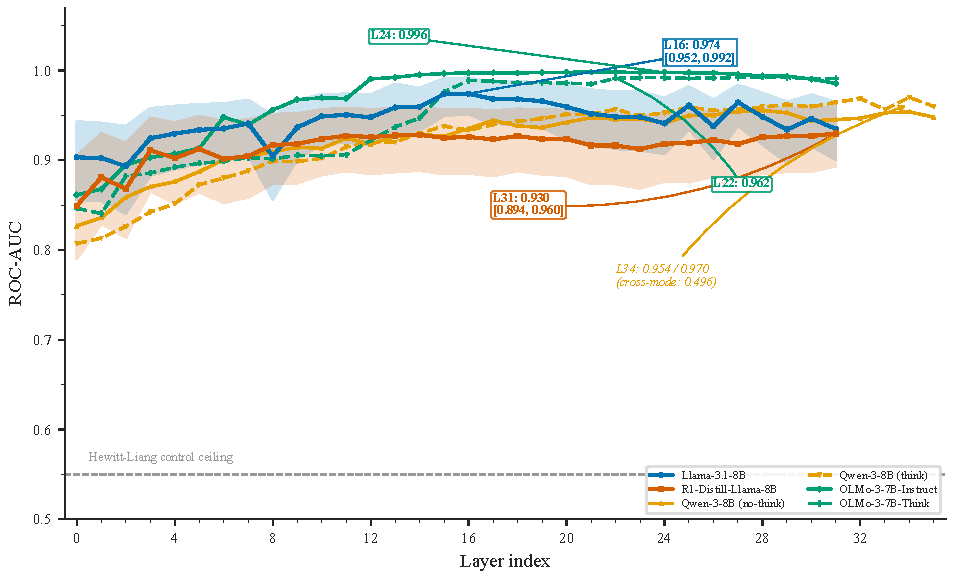
\includegraphics[width=\linewidth]{../figures/fig1_probe_auc_curves.pdf}
\caption{Layer-wise probe ROC-AUC for classifying conflict vs.\
  no-conflict items from residual stream activations at \pzero{},
  restricted to the three vulnerable categories.  Llama-3.1-8B-Instruct
  (blue) peaks at AUC\,=\,0.974 [0.952, 0.992] at L16;
  R1-Distill-Llama-8B (red) peaks at AUC\,=\,0.930 [0.894, 0.960] at
  L31 (CIs overlap slightly but point estimates differ by 0.044).
  Qwen~3-8B no-think (orange solid) peaks at AUC\,=\,0.954 and think
  (orange dashed) at 0.970, both at L34, but cross-mode transfer is
  at chance (0.496).
  Dashed gray line: Hewitt--Liang control task ceiling.}
\label{fig:probe_curves}
\end{figure}

\paragraph{Llama-3.1-8B-Instruct.}  The conflict/control signal builds
rapidly from AUC\,=\,0.85 at layer 0 to AUC\,=\,0.974 at layer 16
(95\% CI [0.952, 0.992]), then remains above 0.95 through layer 31.
The peak at mid-to-upper layers is consistent with prior findings that
mid-network representations encode task-relevant distinctions most
strongly \citep{zhang2025probing}.

\paragraph{R1-Distill-Llama-8B.}  The layer-wise profile is qualitatively
similar---signal builds in early layers---but is \emph{uniformly lower},
peaking at AUC\,=\,0.930 (95\% CI [0.894, 0.960]) at layer 31 (CIs
overlap slightly with Llama's but point estimates differ by 0.044).
The later peak layer (L31 vs.\ L16) suggests
that reasoning distillation shifts conflict-relevant information toward
deeper layers.

\paragraph{Qwen~3-8B (no-think mode).}  Probes on Qwen~3-8B no-think
activations reach peak AUC\,=\,0.954 at layer~34 on the vulnerable
categories, intermediate between Llama (0.974) and R1-Distill (0.930)
and consistent with its intermediate behavioral vulnerability (21.2\% lure
rate).

\paragraph{Qwen~3-8B (think mode).}  Probes on Qwen~3-8B think-mode
activations, extracted at \pzero{} before the
\texttt{<think>} block begins, reach peak
AUC\,=\,0.970 at layer~34.  Despite a 3$\times$ behavioral improvement
(lure rate $21.2\% \to 7.3\%$), cross-mode probe transfer is at chance
(AUC\,=\,0.496, cosine\,=\,$-0.005$), consistent with
\citet{afzal2025knowing}, who showed probes can predict
chain-of-thought success before the first token is generated.
This is the key dissociation: training (Llama vs.\ R1-Distill)
changes both encoding and behavior; inference-time thinking (Qwen no-think
vs.\ think) changes behavior without changing encoding.

\paragraph{Selectivity.}  Hewitt--Liang control probes (trained on
permuted labels) achieve AUC\,$\leq$\,0.66 at all layers for both models,
confirming that the true probes decode representational content, not
probe capacity.  Selectivity exceeds 34 percentage points at peak layers
for both models.\footnote{We report two complementary probe analyses:
  (i)~5-fold CV on all 330 items across 7 categories, which peaks at L14
  with AUC\,=\,0.999 (Llama) and is used for cross-prediction;
  (ii)~bootstrap CI analysis restricted to 160 vulnerable-category items
  (3 categories, 1000 resamples), which peaks at L16 with
  AUC\,=\,0.974 [0.952, 0.992].  The bootstrap analysis provides
  statistical rigor; the all-category analysis provides the direction
  used for cross-prediction and steering.}

\paragraph{Immune category control.}  Probes trained on the four immune
categories (CRT, arithmetic, framing, anchoring) achieve
AUC\,=\,1.0 at layers 0--1 for both models, declining to
AUC\,$\approx$\,0.95 at deeper layers.  This \emph{complicates} the
interpretation: the probes partially detect the presence of lure text
(i.e., the conflict/control distinction in the stimulus itself) rather
than exclusively reflecting the model's processing mode.  We address
this confound in Section~\ref{sec:specificity}.

\subsection{Summary of Probing Results}

Table~\ref{tab:probe_summary} summarizes the key probing metrics.

\begin{table}[t]
\centering
\caption{Probing summary at peak layer for the three
  vulnerable categories.  95\% CIs from 1000 bootstrap resamples
  (Llama and R1-Distill).
  Selectivity = true AUC $-$ control AUC.
  Qwen think and no-think produce identical probe results despite
  a 3$\times$ behavioral difference.  OLMo replicates the same
  direction: Instruct $>$ Think.}
\label{tab:probe_summary}
\vspace{4pt}
\scriptsize
\begin{tabular}{lccccc}
\toprule
\textbf{Model} & \textbf{Pk.\ L} & \textbf{AUC} & \textbf{95\% CI} & \textbf{Ctrl} & \textbf{Sel.} \\
\midrule
Llama-8B-Inst.        & L16 & .974 & [.952, .992] & .63 & .343 \\
R1-Dist.-Llama-8B     & L31 & .930 & [.894, .960] & .55 & .377 \\
Qwen~3-8B (no think)  & L34 & .954 & ---          & --- & 0.496 \\
Qwen~3-8B (think)     & L34 & .970 & ---          & --- & 0.496 \\
\midrule
OLMo-3-7B-Inst.       & L24 & .996 & [.988, 1.000] & --- & --- \\
OLMo-3-7B-Think       & L22 & .962 & [.934, .982]  & --- & --- \\
\bottomrule
\end{tabular}
\end{table}

\subsection{Resolving the Surface-Feature Confound}
\label{sec:specificity}

Probes achieve AUC\,=\,1.0 on behaviorally immune categories (CRT,
arithmetic, framing, anchoring) at early layers, raising the concern
that the conflict/control signal partially reflects surface features of
lure text rather than processing mode.  We resolve this confound with
three converging analyses.

\paragraph{Cross-prediction.}
We train a probe on Llama's \emph{vulnerable} categories (base rate,
conjunction, syllogism) and test it on the \emph{immune} categories
(CRT, arithmetic, framing, anchoring).  If the probe captures a
universal processing-mode signal, it should transfer; if it captures
category-specific lure susceptibility, it should not.  At the peak layer
(L16), the Llama probe achieves transfer AUC\,=\,0.378---below chance
parity and far below the within-category AUC of 0.974.  The probe is
specific to the categories where the model is actually vulnerable.  For
R1-Distill, results are mixed: transfer AUC\,=\,0.878 at L4 (early,
likely surface features) but 0.385 at L31 (late, consistent with
specificity).

\paragraph{Transfer matrix.}
Training probes on each vulnerable category and testing on all others
(Llama, L16) reveals a structured pattern: base rate neglect,
conjunction, and syllogism probes transfer well to each other
(AUC\,$\geq$\,0.950), but CRT probes do not transfer to any vulnerable
category (AUC\,=\,0.062).  This confirms a shared processing-mode
direction across the three vulnerable categories that is absent in
immune categories.

\paragraph{Lure susceptibility scores.}
We extract continuous \pzero{} logit scores for the S1-lure answer on
each conflict item.  Llama's mean lure susceptibility is $+0.422$
(the lure answer is favored in the pre-generation representation),
while R1-Distill's mean is $-0.326$ (the correct answer is favored).
The sign flip confirms that the representational difference is not just
about separability of conflict/control conditions but about the
\emph{direction} of the model's initial commitment: the standard model
leans toward the lure before generation begins; the reasoning model leans
away from it.

\paragraph{Cross-model probe transfer.}
Cross-model transfer further validates the signal: a probe trained on
Llama's vulnerable categories achieves AUC\,=\,0.920 when tested on
R1-Distill's activations at layer~23 (vs.\ within-model AUC of 0.987).
The reverse transfer---R1-Distill to Llama---achieves AUC\,=\,0.954 at
layer~15 (vs.\ self AUC of 0.943).  The \sone{}/\stwo{} processing-mode
direction is substantially shared across models that differ in reasoning
training but share architecture and vocabulary, contrasting with
\citet{huang2026cogbias}'s near-orthogonal finding on architecturally
distinct models.

\subsection{Causal Evidence: Probe-Direction Steering}
\label{sec:results_steering}

We extract the 3-category probe weight vector at L14 (CV AUC\,=\,0.960),
normalize it, and add $\alpha \cdot \hat{\mathbf{w}}$ to the residual
stream continuously during generation, sweeping $\alpha \in \{-5, \ldots, +5\}$
across 80 vulnerable conflict items.

\paragraph{Llama dose-response.}
Steering produces a monotonic 37.5pp causal swing: lure rate rises to
68.8\% at $\alpha\!=\!-5$ (toward \sone{}) and drops to 31.2\% at
$\alpha\!=\!+5$ (toward \stwo{}).  All lure reduction converts to
correct answers (zero ``other'' increase).  Five random-direction controls
show no systematic effect (52--58\% lure across all $\alpha$).

\paragraph{R1-Distill layer sweep.}
We sweep four R1 layers (L14, L25, L28, L31) under continuous
2048-token steering.  No layer produces a coherent dose-response:
lure rate fluctuates between 6--14\% with no monotonic trend.  At
L31 (R1's probe peak), lure is 10.0\% at $\alpha\!=\!-5$ and 11.25\%
at $\alpha\!=\!+5$ (baseline 11.25\%)---a 1.25pp endpoint swing (full
sweep range 5.0pp) versus Llama's 37.5pp endpoint swing.  The model remains fluent (correct rate $\geq$86\%).
The direction is not stably controllable in R1-Distill at any layer:
\emph{readable but not writable}.

\paragraph{Specificity controls.}
Probe steering on matched non-conflict items produces zero lure
responses at any $\alpha$.  The CogBias-style mean-difference vector
(cosine $= 0.314$ with probe) is a stronger one-sided debiasing
intervention (11.25\% lure at $\alpha\!=\!+5$) but is unidirectional;
the probe direction is bidirectional, making it better evidence of a
causal boundary.

\subsection{SAE Features and Attention Entropy}
\label{sec:results_sae}

SAE analysis of Llama's L19 residual stream identified 41 features
with significant conflict/control differential activation (BH-FDR
$q < 0.05$), all surviving Ma et al.\ falsification
\citep{ma2026falsification}.  Attention entropy analysis reveals
R1-Distill has nearly twice as many \stwo{}-specialized heads as Llama
(57 vs.\ 30 of 1024; BH-FDR $q < 0.05$, $|r_{rb}| \geq 0.3$).

% ============================================================
% 5. Discussion
% ============================================================

\section{Discussion}
\label{sec:discussion}

\paragraph{Conflict detection without resolution.}
The central finding maps precisely onto De~Neys' conflict detection
paradigm \citep{deneys2012bias, deneys2017dual}: the standard model
\emph{detects} the conflict between heuristic and normative responses
(AUC\,=\,0.974 at L16) yet \emph{fails to resolve} it (27.3\% lure
rate).  This parallels the human finding that conflict monitoring---indexed
by anterior cingulate cortex activation \citep{botvinick2001conflict,
kerns2004anterior}---often occurs even when the heuristic response
prevails.  Our \pzero{} probe functions analogously to an ACC conflict
signal: it registers the presence of a heuristic--normative tension in
the pre-generation representation, but this tension alone is insufficient
to override the heuristic pathway.  The first-token confidence data
sharpen this parallel: Llama's reduced first-token probability (0.751
vs.\ 0.793) and elevated entropy (0.948 vs.\ 0.817) on conflict items
provide a behavioral analogue of De~Neys' response-time signatures,
confirming that the model's output reflects the internal tension even
before chain-of-thought unfolds.

The reasoning model shows \emph{less} distinct conflict encoding
(AUC\,=\,0.930) yet dramatically better resolution (2.4\% lure rate)---a
pattern confirmed both behaviorally and mechanistically in the OLMo
family (14.9\% $\to$ 0.9\% lure rate; AUC 0.996 $\to$ 0.962, higher
in 30/32 layers), establishing this as a general phenomenon across
architectures.
If reasoning training simply added a ``System~2 module'' that overrides
System~1, we would expect sharper separability.  Instead, the AUC drop
suggests that reasoning distillation makes Type~2 processing
\emph{autonomous}---a phenomenon Evans explicitly predicts:
``Type~2 processes, practiced over time, can become automatic and
default'' \citep{evans2019reflections, evans2013dual}.  On this view,
R1-Distill does not override S1 with S2; it has internalized the
deliberative pathway so thoroughly that it no longer needs a sharp
conflict signal to route items correctly---consistent with evidence
that base models already possess latent reasoning capabilities, with
post-training teaching \emph{when} to deploy them rather than
\emph{how} \citep{venhoff2025base}.  The lure susceptibility scores
confirm this: Llama's pre-generation representation actively favors the
lure ($+0.422$), while R1-Distill's favors the correct answer
($-0.326$).  Reasoning training doesn't just blur a boundary---it
flips the model's default commitment.

\paragraph{Domain-specific vulnerability.}
Three categories are vulnerable (base rate neglect, conjunction fallacy,
syllogisms) while four are immune (CRT, arithmetic, framing, anchoring).
This category-specificity mirrors Stanovich's concept of \emph{dysrationalia}
\citep{stanovich2016rationality}: rational thinking deficits are
domain-specific, not general.  Just as high-IQ humans can fail base rate
problems while acing CRT variants, our models show selective vulnerability
that is specific to certain heuristic families.  The OLMo replication
sharpens this point: OLMo Instruct is vulnerable to loss aversion
(33.3\%) where Llama is immune (0\%), yet both share base rate and
conjunction vulnerability.  Bias profiles are model-specific---a function
of training data and optimization procedure, not architecture---which
means auditing a single model family is insufficient for characterizing
LLM bias susceptibility in general.

\paragraph{Ecological rationality and format dependence.}
A preliminary test of Gigerenzer's ecological rationality critique
\citep{gigerenzer1995improve} yielded an unexpected reversal: natural
frequency framing \emph{increased} lure susceptibility in both models
(Llama: $84\% \to 100\%$; R1-Distill: $4\% \to 40\%$), suggesting
that LLM bias sensitivity is format-dependent in ways that diverge from
human cognition, where natural frequencies reliably \emph{reduce}
base rate neglect.  This inversion warrants systematic investigation
across all bias categories and models.

\paragraph{Training vs.\ inference.}
Qwen's think/no-think result is the sharpest finding: thinking mode
reduces lure rates from 21.2\% to 7.3\% on the same weights, yet probes
reach similar peak AUC in both modes (0.954 no-think, 0.970 think at L34) yet cross-mode transfer is at chance.  The toggle
changes what the model \emph{does} during generation, not what it
\emph{encodes} at \pzero{}.  Combined with the Llama/R1-Distill comparison
(where training \emph{does} change encoding: 0.974 $\to$ 0.930), this
yields a clean dissociation: \textbf{training changes \sone{}/\stwo{}
encoding; inference-time thinking changes \sone{}/\stwo{} behavior
without changing encoding.}

This parallels the neuroscience distinction between structural and
functional plasticity \citep{kolb2013brain}: training rewires the weights
so that P0 favors the normative answer; inference-time thinking adapts
the activation pattern on an unchanged structural substrate.  This is
consistent with \citet{ziabari2025reasoning} and
\citet{codaforno2025dual}'s overlapping subspaces, but adds a new
dimension: the encoding/behavior dissociation reveals two distinct
mechanisms for bias resistance, not one.

\paragraph{Specificity.}
Cross-prediction (Section~\ref{sec:specificity}) resolves the
surface-feature confound: Llama's vulnerable-category probe yields
transfer AUC\,=\,0.378 on immune categories, and the transfer matrix
shows vulnerable categories share a processing-mode direction
(mutual AUC\,$\geq$\,0.950) absent in CRT (AUC\,=\,0.062).
Cross-model transfer (Llama$\to$R1: 0.920; R1$\to$Llama: 0.954)
confirms that this direction is shared across reasoning-differentiated
models, not model-specific.  The probe captures how the model processes
lures, not that lures are present.

\paragraph{Readable but not writable.}
In Llama, the probe direction is readable (AUC\,=\,0.974) and writable
(37.5pp bidirectional causal swing); in R1-Distill, it is readable
(AUC\,=\,0.930) but not detectably writable at any layer (L14--L31)
under continuous intervention.  The layer sweep rules out the hypothesis
that the writable locus simply moved deeper.  The bias direction in
R1-Distill is in this sense \emph{vestigial}---an echo of pre-training
representations that reasoning distillation has decoupled from the
behavioral output pathway.  This dissociation is direct evidence for
Evans' S2-by-default hypothesis \citep{evans2019reflections}.

\paragraph{Relation to CogBias.}
\citet{huang2026cogbias} showed that bias directions are steerable
(26--32\% bias reduction via mean-difference vectors); we show that
reasoning post-training decouples the same directions from behavioral
control.  We extend CogBias via cross-model transfer (shared direction
when architecture is held constant, AUC\,$>$\,0.92), a within-model
toggle (Qwen), and layer-sweep steering to establish causal
dissociation.

\paragraph{Methodological safeguards.}
Probing can produce plausible results even on random networks
\citep{meloux2025dead}, and SAE features often fail falsification
\citep{sanitychecks2026}.  We address this five ways: (1)~Hewitt--Liang
controls (Section~\ref{sec:probes}) show selectivity $>$34pp;
(2)~cross-prediction (Section~\ref{sec:specificity}) provides structural
falsification---noise probes would not systematically drop to
AUC\,=\,0.378 on immune categories; (3)~the inter-model comparison is
itself a control---identical prompts yield different AUCs (0.974
vs.\ 0.930) only if the models encode inputs differently;
(4)~cross-model probe transfer (AUC\,$>$\,0.92) confirms the signal is
not model-specific but reflects a shared representational direction;
(5)~all 41 SAE features survive Ma et al.\ falsification
(Section~\ref{sec:results_sae}), with zero spurious features after
token-injection testing.

\paragraph{Limitations.}
(i) Model scale: all models are 7--8B parameters; the blurring effect
may manifest differently at 70B+.  Cross-architecture replication
(Llama and OLMo families) mitigates concern about architecture-specific
artifacts but does not address scale.
(ii) Linear probes may miss nonlinear representational structure; MLP
probes and CCS \citep{burns2022discovering} are planned robustness checks.
(iii) We measure conflict/control separability, which is a proxy for
\sone{}/\stwo{} processing mode---not a direct readout of ``how the model
is thinking.''
(iv) The Qwen think-mode \pzero{} position is pre-think; probing
\emph{within} the thinking trace (T0 through Tend) would reveal whether
representations shift during chain-of-thought.

\paragraph{Future work.}
SAE analysis has identified 41 falsification-surviving features that
differentiate conflict and control processing
(Section~\ref{sec:results_sae}).  The natural next step is
\textbf{causal interventions}: steer these features in the standard
model to test whether artificially blurring the \sone{}/\stwo{}
boundary improves bias resistance without chain-of-thought cost, and
conversely, whether sharpening the boundary in the reasoning model
reintroduces vulnerability.

% ============================================================
% Acknowledgments (anonymized for review)
% ============================================================

\section*{Acknowledgments}

\emph{Omitted for double-blind review.}

% ============================================================
% References
% ============================================================

\bibliographystyle{plainnat}
\bibliography{references}

\end{document}
